\documentclass[9pt]{pnas-new}
% Use the lineno option to display guide line numbers if required.
% Note that the use of elements such as single-column equations
% may affect the guide line number alignment. 

%\RequirePackage[english,slovene]{babel} % when writing in slovene
%\RequirePackage[slovene,english]{babel} % when writing in english

\templatetype{pnasresearcharticle} % Choose template 
% {pnasresearcharticle} = Template for a two-column research article
% {pnasmathematics} = Template for a one-column mathematics article
% {pnasinvited} = Template for a PNAS invited submission

%\selectlanguage{slovene}
%\etal{in sod.} % comment out when writing in english
%\renewcommand{\Authands}{ in } % comment out when writing in english
%\renewcommand{\Authand}{ in } % comment out when writing in english

\newcommand{\set}[1]{\ensuremath{\mathbf{#1}}}
\renewcommand{\vec}[1]{\ensuremath{\mathbf{#1}}}
\newcommand{\uvec}[1]{\ensuremath{\hat{\vec{#1}}}}
\newcommand{\const}[1]{{\ensuremath{\kappa_\mathrm{#1}}}} 

\newcommand{\num}[1]{#1}

\graphicspath{{./fig/}}

\title{Nest-site selection in mass-recruiting ant species}

% Use letters for affiliations, numbers to show equal authorship (if applicable) and to indicate the corresponding author
\author{Meggy-Lie-Anne Chamand}
\author{Kim Georget}
\author{Bella Muradian}
\author{Clara Stavun}

\affil{Collective behaviour course research seminar report} 

% Please give the surname of the lead author for the running footer
\leadauthor{Chamand} 

\selectlanguage{english}


% Please add here a significance statement to explain the relevance of your work
\significancestatement{Programmable modeling environment}{To solve the problem written above, we will use an agent-based model built in NetLogo. NetLogo is a widely used, user-friendly agent-based modeling environment tailored for simulating complex systems, making it ideal for studying ant social behavior and collective decision-making with its visual interface and real-time simulations.

It's worth noting that the NetLogo platform, while effective for simulating ant behavior, has limitations, especially in terms of visual representation. We could only use basic shapes (circles, triangles, stars) in limited colors to represent our elements (food, predators, protection). 
}

\selectlanguage{english}

% Please include corresponding author, author contribution and author declaration information
%\authorcontributions{Please provide details of author contributions here.}
%\authordeclaration{Please declare any conflict of interest here.}
%\equalauthors{\textsuperscript{1}A.O.(Author One) and A.T. (Author Two) contributed equally to this work (remove if not applicable).}
%\correspondingauthor{\textsuperscript{2}To whom correspondence should be addressed. E-mail: author.two\@email.com}

% Keywords are not mandatory, but authors are strongly encouraged to provide them. If provided, please include two to five keywords, separated by the pipe symbol, e.g:
\keywords{Agent-based model | New nest-site choice | Mass-recruiting ant | Quorum | simulation} 

\begin{abstract}
This study explores the intricate behavior of ant colonies, focusing on the nest emigration process of the M.nipponica ant. Using an agent-based model, we study the collective decision-making of ants during nest-site selection. We focus on finding the best possible nest while introducing new parameters meant to influence the quality of a given nest (i.e. food, protection, predator). Through simulations, we assessed the impact of two parameters - quorum percent and commitment base - on the speed and the accuracy of their choice, and for each parameter, we were able to find a range for which the efficiency of the ants were optimized. 
\end{abstract}

\dates{\textbf{\today}}
\program{BM-RI}
\vol{2023/24}
\no{CB:H} % group ID
%\fraca{FRIteza/201516.130}

\begin{document}

% Optional adjustment to line up main text (after abstract) of first page with line numbers, when using both lineno and twocolumn options.
% You should only change this length when you've finalised the article contents.
\verticaladjustment{-2pt}

\maketitle
\thispagestyle{firststyle}
\ifthenelse{\boolean{shortarticle}}{\ifthenelse{\boolean{singlecolumn}}{\abscontentformatted}{\abscontent}}{}

% If your first paragraph (i.e. with the \dropcap) contains a list environment (quote, quotation, theorem, definition, enumerate, itemize...), the line after the list may have some extra indentation. If this is the case, add \parshape=0 to the end of the list environment.
\dropcap{S}ocial insects have simple yet captivating individuals and thus provide an ideal subject for scientific exploration. This study delves into the intricate behavior of ant colonies, particularly during the emigration process to new nests, with a specific focus on the nest emigration process of the M. nipponica ant. Our research aims to unravel the complexities of ant colony behavior in the context of new nest selection, by examining various parameters, including the quorum percent, commitment base, and pheromone deposition, to understand their collective role in decision-making.

While significant strides have been made in understanding ant colonies, certain aspects, such as behavioral rules, remain elusive. Simultaneously, existing models contribute to giving valuable insights into how ants collectively decide on nest-site selection. For instance, mass-recruiting algorithms emulate complex collective biological processes \cite{computational_model}, while quorum-sensing mechanisms rely on cumulative pheromone thresholds for nest-site selection \cite{quorum_sensing_recruitment}. Additionally, models consider variable acceptance thresholds, reflecting diverse ant preferences, and individual assessment behavior, where some ants prioritize proximity to food sources, while others favor concealment from predators \cite{variability_individual_assessment}.

However, existing models often focus on specific parameters, hindering a comprehensive assessment of their relative influence. In response, our research adopts a holistic approach, integrating multiple parameters to elucidate their collective impact on decision-making processes during nest emigration. The paper we selected aimed to contribute to a more nuanced understanding of the intricate dynamics within ant colonies during new nest selection, by trying to determine how ants choose one ‘good’ nest amongst ‘bad’ by replicating as well as possible the ants' behavior \cite{agent_based_model}. We took a step further and changed this model to study the ability of ants to choose the ‘best’ nest amongst a pool of acceptable nests to be more applicable to other areas   


\section*{Method}
\subsection*{Model set up}
The initial model represented ant nests and their movements, with each nest varying in shape, size, position, and assigned a random quality number. Nests higher a user-defined quality threshold are deemed good (yellow), while others are bad (orange). Users can visualize both nest configurations and ant activities.

In the improved version, users can add three factors near each nest: food (purple square), protection (yellow star), and predators (red triangle), influencing nest quality. The default quality is 50 points, altered by the presence of these elements. The presence of food or protection each adds 20 points, while a predator deducts 30 points. In consequence, nest quality can range from 20 (only predator) to 90 (food and protection, no predator).

 
\begin{figure}[h!tbp]
	\centering
	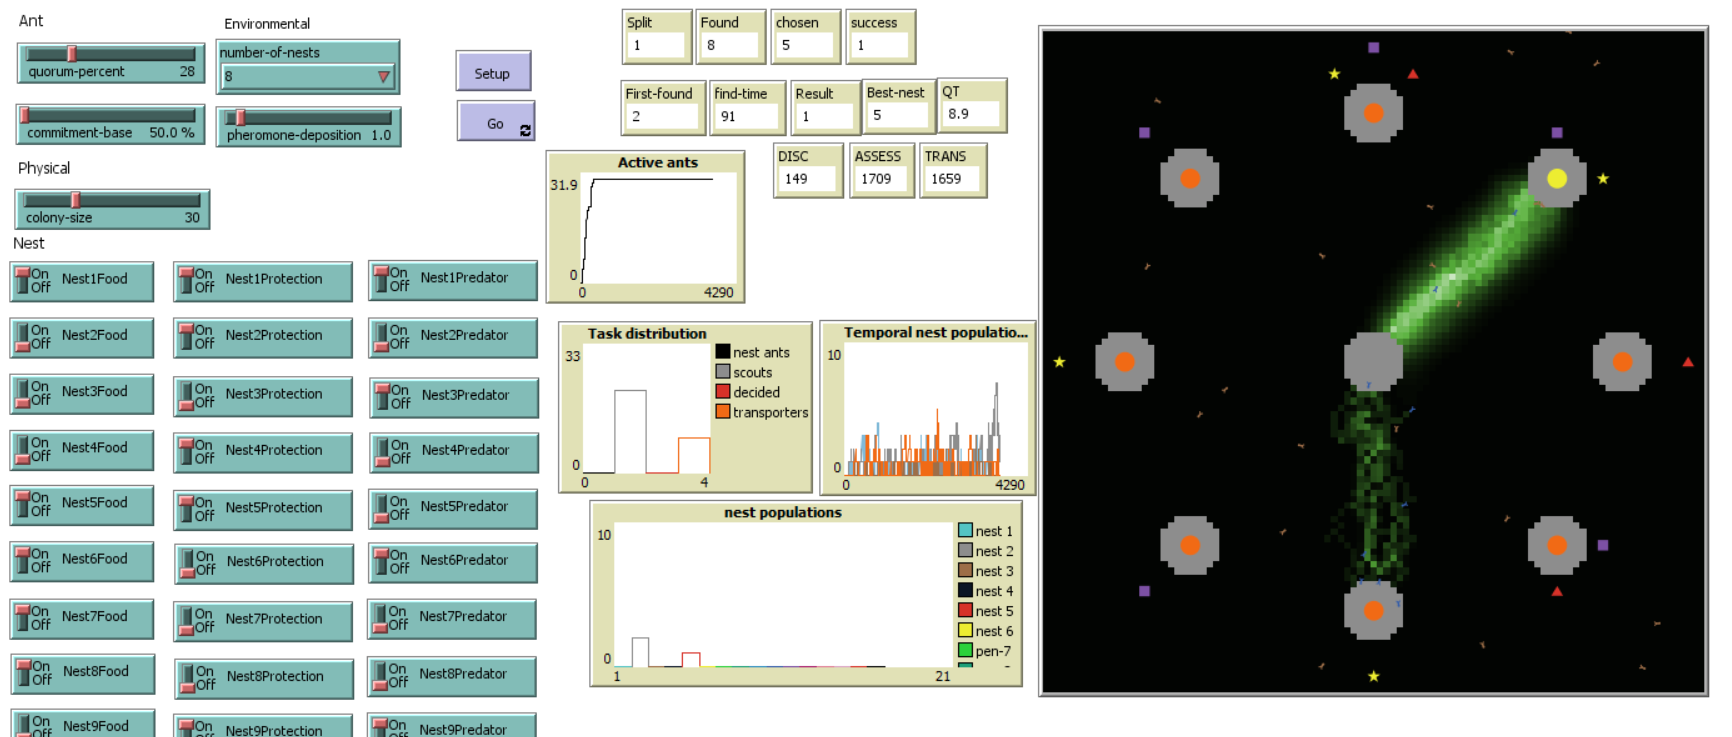
\includegraphics[width=.9\linewidth]{report-template/fig/netlogo.png}
	\caption{Model setup screenshot on NetLogo. On the left: the settings that the user can modify. In the middle: the obtained results. On the right: the real-time visualization of the simulation}
	\label{fig:netlogo}
\end{figure}
The interface allows users to customize simulations by selecting nest size, shape, and parameters like food, protection, or predators, with each nest's quality calculated automatically (on the left).

During the simulation, ant movements are visible on the right side. Nest turn yellow if they are classified as good and orange if bad. Pheromone trails are shown as green or white lines, indicating quantity.

Results are displayed in the center, showing real-time ant quantities (as detailed in the implementation) and, upon completion, the simulation's success and the selected nest.



\subsection*{Implementation}



The colony's goal is to locate the best nest, involving two key agents: nests and ants.
\begin{itemize}

    \item Nests : Each nest has a quality number (20 to 90) defining its class as "good" or "bad." The default assumption is that all nests are good, and the objective is to have ants classify all nests as bad, except for the one with the highest quality.  Each nest tracks the number of ant visits, which is used to check if the quorum (an ant parameter) is reached.
    
    \item Ants : They possess various parameters. Ants are able to memorize the position of the original and chosen (when they find a suitable one) nests. They can either move randomly or go towards nests with known positions. An internal threshold (default: 50) classifies discovered nests as good or bad ; its value is set to the highest quality value of discovered nests. Ants share a quorum parameter for final nest validation before colony relocation.
\end{itemize}

During the simulation, four ant types emerge:

\begin{itemize}
    \item Nest ants: Remain in the original nest until transitioning to become scout ants.
    \item Scout ants: Explore the area randomly or follow pheromone trails to evaluate the nests. If a discovered nest is initially good, they reevaluate it; if it becomes bad, they continue exploring. If it’s good, they become ‘decided’ ants and save this nest as the ‘chosen nest’. 
    \item Decided ants: When an ant identifies a potential good nest, it goes back and forth between the original and chosen nest. Each time it reaches the chosen nest, it checks whether it has been classified as bad; if so, it goes back to being a ‘scout’ ant, otherwise, it checks whether the quorum has been reached. If this is the case, the ant becomes a transport ant; otherwise, it continues walking between the two nests potentially reverting to scouts based on the "commitment-based" parameter.
    \item Transport ants: Move between the chosen and original nests, transporting brood until the relocation is complete."
\end{itemize}
  (Figure \ref{fig:implementdiag}) The ants' general behavior in this model is influenced by several parameters. We decided to focus on two specific parameters:
\subsubsection*{The quorum percent}, which represents the percentage of ants needed to visit a good nest for it to be chosen by the colony.
\subsubsection*{The commitment base} influences the probability of an ant reverting to being a scout after deciding on a nest.
\begin{figure}[h!tbp]
    \centering
    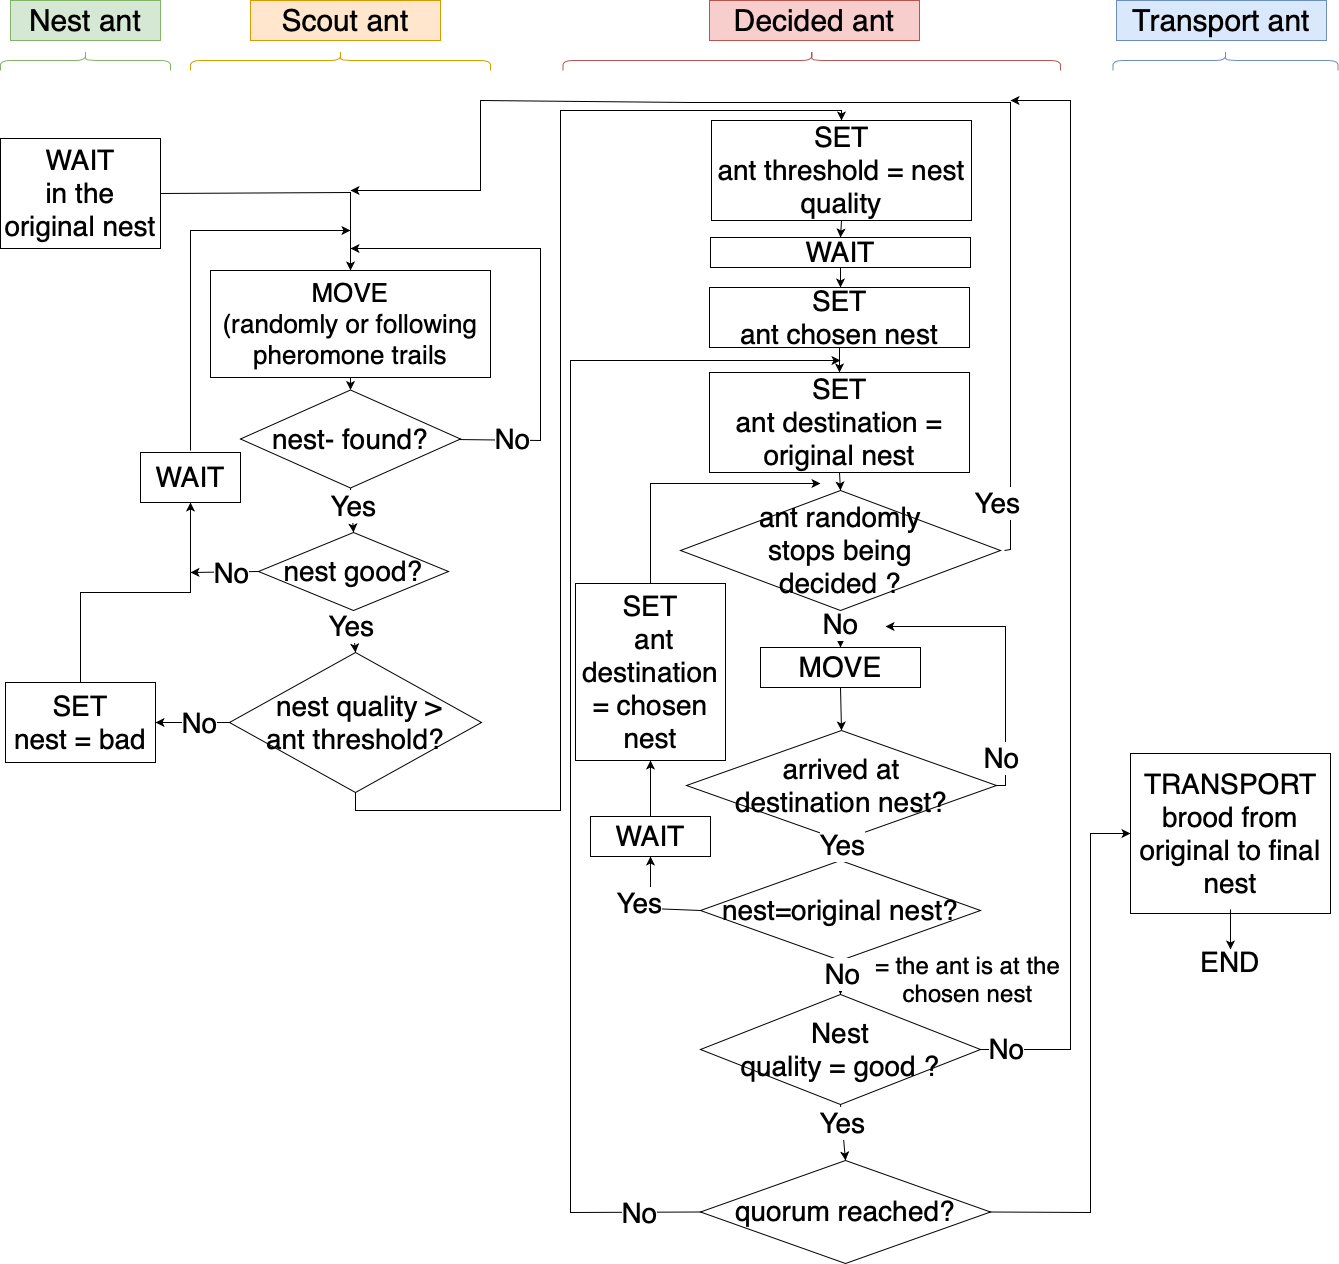
\includegraphics[width=1\linewidth]{report-template/fig/implementation.png}
    \caption{Simplified diagram of the model implementation algorithm}
    \label{fig:implementdiag}
\end{figure}

\section*{Tests and validation}
After validating our code, we conducted simulations to assess how well our model guides ants to the optimal nest under varied parameters. Previous tests indicated that pheromone deposition did not have a significant impact, leading us to focus specifically on quorum percent and commitment-base percentage. Quorum percent signifies the minimum ant participation for nest selection, while commitment base influences the likelihood of an ant reverting to scouting after nest selection.\\ 
Testing different parameter combinations across nest configurations allowed us to evaluate ants' nest-finding abilities in diverse environments. Our aim was to find optimal values for these parameters, that would be able to ensure consistent discovery of the best nests. Our simulations’ values of parameters followed the default values from the initial paper ; we changed only in the parameters under investigation. For each simulation, we opted for a colony of 60 ants, aligning with the average colony size of the studied species (M. nipponica).





\section*{Results}
From the different simulation setups we ran, we formed different conclusions according to the results we obtained. 

\subsubsection*{Ants overall decisions}
In this model, the ants tend to get better results than in the model from the previous report (in the previous report, the ants didn't reassess their chosen nest class once they became "decided ants"). They rarely choose a bad nest, however, they take more time to choose a final nest, so since there is a time limit on the simulation, they regularly don't reach the needed quorum in time.


\subsubsection*{Commitment base}
\\The commitment base's influence primarily affects the ants' ability to find the correct nest in time. They rarely choose a bad nest, validating the model's implementation
\\Good results occur when the commitment base is between 50\% and 98.9\% and there are 1 to 8 nests, as ants often migrate to the best nest. However, with a low commitment base, ants struggle to choose quickly due to insufficient time as decided ants. The best performance, with ants consistently finding the best nest quickly, is seen with a high commitment base of 98\% to 98.9\%. For 16 nests, this range still performs well, but lower values lead to delayed decisions.
\\A commitment base of 99\% or higher is too high, causing ants to choose the first good nest too quickly and not reach a quorum in a reasonable time.
\\Thus, the optimal commitment base range is 98\% to 98.9\%, which also results in shorter average simulation times.
\begin{figure}[h!tbp]
    \begin{minipage}[c]{.46\linewidth}
        \centering
        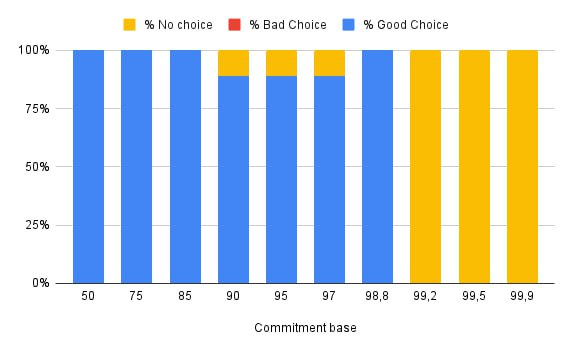
\includegraphics[width=0.95\textwidth]{report-template/fig/commit_bar.jpeg}
        \caption{Proportion of Good choice, Bad choice and No choice for different values of commitment-base, in a 8 nests environment}
        \label{fig:vr8}
    \end{minipage}
    \hfill%
    \begin{minipage}[c]{.46\linewidth}
        \centering
        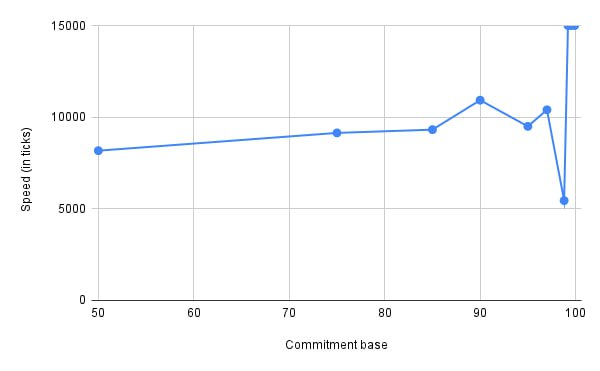
\includegraphics[width=0.95\textwidth]{report-template/fig/commit_diag.jpeg}
        \caption{Average speed of choice of the best nest according to the commitment-base values}
        \label{fig:c8}
    \end{minipage}
\end{figure} 
\subsubsection*{Quorum percent}
\\As stated in a previous section, the quorum percent is the needed percentage of ants visiting a good nest for it to be chosen by the colony. We established that the quorum should be set between 25\% and 50\%, depending on the complexity of the environment. Here we wanted to assert this statement so we tested more values of this parameter. 
With our new set of simulations, we were able to refine this interval and found out that the ants were able to choose the ‘best nest’ when the quorum was in the interval [30\%, 45\%].
This interval has also been chosen because the simulation time is shorter for these values.

\begin{figure}[h]
    \begin{minipage}[c]{.46\linewidth}
        \centering
        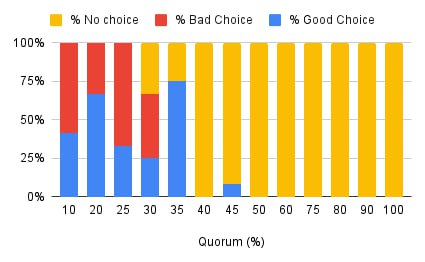
\includegraphics[width=0.95\textwidth]{report-template/fig/quorum_bar.jpeg}
        \caption{Proportion of Good choice, Bad choice and No choice for different values of quorum-percent, in a 8 nests environment}
        \label{fig:vr8}
    \end{minipage}
    \hfill%
    \begin{minipage}[c]{.46\linewidth}
        \centering
        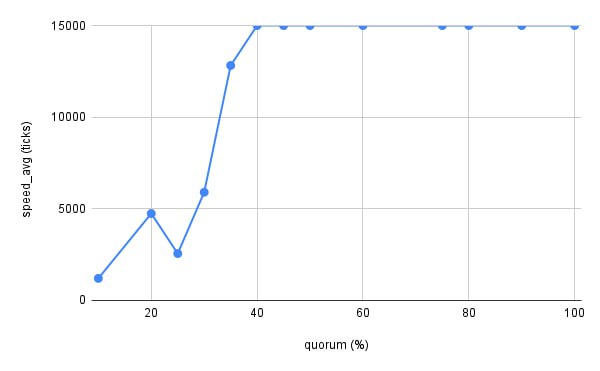
\includegraphics[width=0.95\textwidth]{report-template/fig/quorum_diag.jpeg}
        \caption{Average speed of choice of the best nest according to the quorum-percent values}
        \label{fig:c8}
    \end{minipage}
\end{figure}

\section*{Discussion}
In our study, the behavior model of M. nipponica ants shows significant promise for applications beyond biological research, particularly in fields like robotics and rescue missions. The ant colony's decision-making mechanisms, when adapted, could significantly improve the efficiency of robotic swarms in unknown environments, and optimize rescue teams' strategies in disaster scenarios. However, the model's current constraint of nest placement (centered around the original nest) should evolve to include randomness, better representing real-world unpredictability. This enhancement would not only make the model more environmentally valid but also expand its utility in real-life situations, demonstrating the extensive possibilities of our findings.



\section*{Conclusion}
This research on the nest emigration behavior of M. nipponica ants has yielded insights with far-reaching implications. By delving into the collective decision-making processes of ant colonies and refining existing models to include key parameters like quorum percent and commitment base, we have uncovered nuanced dynamics that govern how these insects handle complex challenges. The study's advancements not only contribute significantly to our understanding of social insect behavior but also open up exciting possibilities for cross-disciplinary applications, particularly in robotics and emergency response strategies. The model's potential in simulating and enhancing decision-making processes in these fields is particularly promising.


 
\acknow{ Meggy C.: tests, slides and report; Kim G.: tests, slides and report, Bella M.: tests; Clara S.: implementation, tests, slides and report.}
\showacknow % Display the acknowledgments section

% \pnasbreak splits and balances the columns before the references.
% If you see unexpected formatting errors, try commenting out this line
% as it can run into problems with floats and footnotes on the final page.
%\pnasbreak

\section*{\bibname}
\bibliographystyle{plain}
\bibliography{report-template/bib/bibliography}

\end{document}